\documentclass[twoside]{book}

% Packages required by doxygen
\usepackage{fixltx2e}
\usepackage{calc}
\usepackage{doxygen}
\usepackage[export]{adjustbox} % also loads graphicx
\usepackage{graphicx}
\usepackage[utf8]{inputenc}
\usepackage{makeidx}
\usepackage{multicol}
\usepackage{multirow}
\PassOptionsToPackage{warn}{textcomp}
\usepackage{textcomp}
\usepackage[nointegrals]{wasysym}
\usepackage[table]{xcolor}

% Font selection
\usepackage[T1]{fontenc}
\usepackage[scaled=.90]{helvet}
\usepackage{courier}
\usepackage{amssymb}
\usepackage{sectsty}
\renewcommand{\familydefault}{\sfdefault}
\allsectionsfont{%
  \fontseries{bc}\selectfont%
  \color{darkgray}%
}
\renewcommand{\DoxyLabelFont}{%
  \fontseries{bc}\selectfont%
  \color{darkgray}%
}
\newcommand{\+}{\discretionary{\mbox{\scriptsize$\hookleftarrow$}}{}{}}

% Page & text layout
\usepackage{geometry}
\geometry{%
  a4paper,%
  top=2.5cm,%
  bottom=2.5cm,%
  left=2.5cm,%
  right=2.5cm%
}
\tolerance=750
\hfuzz=15pt
\hbadness=750
\setlength{\emergencystretch}{15pt}
\setlength{\parindent}{0cm}
\setlength{\parskip}{3ex plus 2ex minus 2ex}
\makeatletter
\renewcommand{\paragraph}{%
  \@startsection{paragraph}{4}{0ex}{-1.0ex}{1.0ex}{%
    \normalfont\normalsize\bfseries\SS@parafont%
  }%
}
\renewcommand{\subparagraph}{%
  \@startsection{subparagraph}{5}{0ex}{-1.0ex}{1.0ex}{%
    \normalfont\normalsize\bfseries\SS@subparafont%
  }%
}
\makeatother

% Headers & footers
\usepackage{fancyhdr}
\pagestyle{fancyplain}
\fancyhead[LE]{\fancyplain{}{\bfseries\thepage}}
\fancyhead[CE]{\fancyplain{}{}}
\fancyhead[RE]{\fancyplain{}{\bfseries\leftmark}}
\fancyhead[LO]{\fancyplain{}{\bfseries\rightmark}}
\fancyhead[CO]{\fancyplain{}{}}
\fancyhead[RO]{\fancyplain{}{\bfseries\thepage}}
\fancyfoot[LE]{\fancyplain{}{}}
\fancyfoot[CE]{\fancyplain{}{}}
\fancyfoot[RE]{\fancyplain{}{\bfseries\scriptsize Generated by Doxygen }}
\fancyfoot[LO]{\fancyplain{}{\bfseries\scriptsize Generated by Doxygen }}
\fancyfoot[CO]{\fancyplain{}{}}
\fancyfoot[RO]{\fancyplain{}{}}
\renewcommand{\footrulewidth}{0.4pt}
\renewcommand{\chaptermark}[1]{%
  \markboth{#1}{}%
}
\renewcommand{\sectionmark}[1]{%
  \markright{\thesection\ #1}%
}

% Indices & bibliography
\usepackage{natbib}
\usepackage[titles]{tocloft}
\setcounter{tocdepth}{3}
\setcounter{secnumdepth}{5}
\makeindex

% Hyperlinks (required, but should be loaded last)
\usepackage{ifpdf}
\ifpdf
  \usepackage[pdftex,pagebackref=true]{hyperref}
\else
  \usepackage[ps2pdf,pagebackref=true]{hyperref}
\fi
\hypersetup{%
  colorlinks=true,%
  linkcolor=blue,%
  citecolor=blue,%
  unicode%
}

% Custom commands
\newcommand{\clearemptydoublepage}{%
  \newpage{\pagestyle{empty}\cleardoublepage}%
}

\usepackage{caption}
\captionsetup{labelsep=space,justification=centering,font={bf},singlelinecheck=off,skip=4pt,position=top}

%===== C O N T E N T S =====

\begin{document}

% Titlepage & ToC
\hypersetup{pageanchor=false,
             bookmarksnumbered=true,
             pdfencoding=unicode
            }
\pagenumbering{alph}
\begin{titlepage}
\vspace*{7cm}
\begin{center}%
{\Large Same Game \\[1ex]\large Beta }\\
\vspace*{1cm}
{\large Generated by Doxygen 1.8.13}\\
\end{center}
\end{titlepage}
\clearemptydoublepage
\pagenumbering{roman}
\tableofcontents
\clearemptydoublepage
\pagenumbering{arabic}
\hypersetup{pageanchor=true}

%--- Begin generated contents ---
\chapter{Hierarchical Index}
\section{Class Hierarchy}
This inheritance list is sorted roughly, but not completely, alphabetically\+:\begin{DoxyCompactList}
\item \contentsline{section}{same.\+Jugar\+Logica}{\pageref{classsame_1_1_jugar_logica}}{}
\item Application\begin{DoxyCompactList}
\item \contentsline{section}{same.\+Jugar\+Interfaz}{\pageref{classsame_1_1_jugar_interfaz}}{}
\item \contentsline{section}{same.\+Menu}{\pageref{classsame_1_1_menu}}{}
\end{DoxyCompactList}
\item Event\+Handler\begin{DoxyCompactList}
\item \contentsline{section}{same.\+Jugar\+Interfaz}{\pageref{classsame_1_1_jugar_interfaz}}{}
\item \contentsline{section}{same.\+Menu}{\pageref{classsame_1_1_menu}}{}
\end{DoxyCompactList}
\end{DoxyCompactList}

\chapter{Class Index}
\section{Class List}
Here are the classes, structs, unions and interfaces with brief descriptions\+:\begin{DoxyCompactList}
\item\contentsline{section}{\hyperlink{classsame_1_1_jugar_interfaz}{same.\+Jugar\+Interfaz} }{\pageref{classsame_1_1_jugar_interfaz}}{}
\item\contentsline{section}{\hyperlink{classsame_1_1_jugar_logica}{same.\+Jugar\+Logica} }{\pageref{classsame_1_1_jugar_logica}}{}
\item\contentsline{section}{\hyperlink{classsame_1_1_menu}{same.\+Menu} }{\pageref{classsame_1_1_menu}}{}
\end{DoxyCompactList}

\chapter{Class Documentation}
\hypertarget{classsame_1_1_jugar_interfaz}{}\section{same.\+Jugar\+Interfaz Class Reference}
\label{classsame_1_1_jugar_interfaz}\index{same.\+Jugar\+Interfaz@{same.\+Jugar\+Interfaz}}
Inheritance diagram for same.\+Jugar\+Interfaz\+:\begin{figure}[H]
\begin{center}
\leavevmode
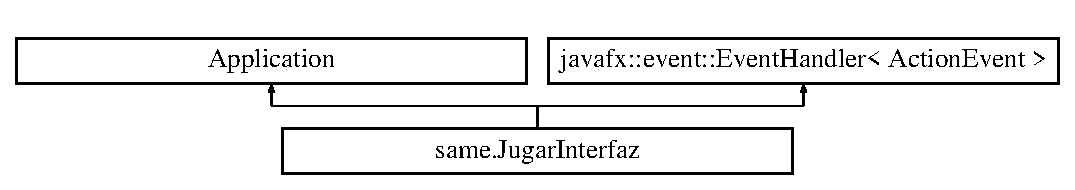
\includegraphics[height=2.000000cm]{classsame_1_1_jugar_interfaz}
\end{center}
\end{figure}
\subsection*{Public Member Functions}
\begin{DoxyCompactItemize}
\item 
void \hyperlink{classsame_1_1_jugar_interfaz_a36f21d8cd6ccb7f9984c09659ec5b35f}{start} (Stage ventana, int nivel)  throws Exception 
\item 
void \hyperlink{classsame_1_1_jugar_interfaz_a9ec4401f9c331df554db86938ccf50b8}{Cambiar\+Estado\+Botones} (Image\mbox{[}$\,$\mbox{]}\mbox{[}$\,$\mbox{]}logico)
\item 
void \hyperlink{classsame_1_1_jugar_interfaz_a81b2d95f6748dfe787b9b72e76a81aca}{Mostrar\+Cambio} (Image\mbox{[}$\,$\mbox{]}\mbox{[}$\,$\mbox{]} logico, Button\mbox{[}$\,$\mbox{]}\mbox{[}$\,$\mbox{]} botones)
\item 
void \hyperlink{classsame_1_1_jugar_interfaz_a917ce15a363f79c0d7428578cb36b85c}{handle} (Action\+Event arg0)
\item 
void \hyperlink{classsame_1_1_jugar_interfaz_ac8c1c753ea40ce008a638af34e91aeda}{start} (Stage primary\+Stage)  throws Exception 
\end{DoxyCompactItemize}
\subsection*{Public Attributes}
\begin{DoxyCompactItemize}
\item 
\mbox{\Hypertarget{classsame_1_1_jugar_interfaz_a9058f937d1cd0d18eb627e30ee93bbe2}\label{classsame_1_1_jugar_interfaz_a9058f937d1cd0d18eb627e30ee93bbe2}} 
Image \mbox{[}$\,$\mbox{]}\mbox{[}$\,$\mbox{]} {\bfseries arreglo\+\_\+logico} = new Image\mbox{[}10\mbox{]}\mbox{[}12\mbox{]}
\item 
\mbox{\Hypertarget{classsame_1_1_jugar_interfaz_a6899655aaf4fe3b0da53d2b22feedec5}\label{classsame_1_1_jugar_interfaz_a6899655aaf4fe3b0da53d2b22feedec5}} 
Button \mbox{[}$\,$\mbox{]}\mbox{[}$\,$\mbox{]} {\bfseries arreglo\+\_\+interfaz} = new Button\mbox{[}10\mbox{]}\mbox{[}12\mbox{]}
\end{DoxyCompactItemize}


\subsection{Member Function Documentation}
\mbox{\Hypertarget{classsame_1_1_jugar_interfaz_a9ec4401f9c331df554db86938ccf50b8}\label{classsame_1_1_jugar_interfaz_a9ec4401f9c331df554db86938ccf50b8}} 
\index{same\+::\+Jugar\+Interfaz@{same\+::\+Jugar\+Interfaz}!Cambiar\+Estado\+Botones@{Cambiar\+Estado\+Botones}}
\index{Cambiar\+Estado\+Botones@{Cambiar\+Estado\+Botones}!same\+::\+Jugar\+Interfaz@{same\+::\+Jugar\+Interfaz}}
\subsubsection{\texorpdfstring{Cambiar\+Estado\+Botones()}{CambiarEstadoBotones()}}
{\footnotesize\ttfamily void same.\+Jugar\+Interfaz.\+Cambiar\+Estado\+Botones (\begin{DoxyParamCaption}\item[{Imagelogico}]{\mbox{[}$\,$\mbox{]}\mbox{[}$\,$\mbox{]} }\end{DoxyParamCaption})}

Cambia las imágenes de la matriz de interfacez al nuevo del lógico 
\begin{DoxyParams}{Parameters}
{\em matriz} & Arreglo lógico que será el encargado de los cambios\\
\hline
\end{DoxyParams}
\mbox{\Hypertarget{classsame_1_1_jugar_interfaz_a917ce15a363f79c0d7428578cb36b85c}\label{classsame_1_1_jugar_interfaz_a917ce15a363f79c0d7428578cb36b85c}} 
\index{same\+::\+Jugar\+Interfaz@{same\+::\+Jugar\+Interfaz}!handle@{handle}}
\index{handle@{handle}!same\+::\+Jugar\+Interfaz@{same\+::\+Jugar\+Interfaz}}
\subsubsection{\texorpdfstring{handle()}{handle()}}
{\footnotesize\ttfamily void same.\+Jugar\+Interfaz.\+handle (\begin{DoxyParamCaption}\item[{Action\+Event}]{arg0 }\end{DoxyParamCaption})}

No hace nada\mbox{\Hypertarget{classsame_1_1_jugar_interfaz_a81b2d95f6748dfe787b9b72e76a81aca}\label{classsame_1_1_jugar_interfaz_a81b2d95f6748dfe787b9b72e76a81aca}} 
\index{same\+::\+Jugar\+Interfaz@{same\+::\+Jugar\+Interfaz}!Mostrar\+Cambio@{Mostrar\+Cambio}}
\index{Mostrar\+Cambio@{Mostrar\+Cambio}!same\+::\+Jugar\+Interfaz@{same\+::\+Jugar\+Interfaz}}
\subsubsection{\texorpdfstring{Mostrar\+Cambio()}{MostrarCambio()}}
{\footnotesize\ttfamily void same.\+Jugar\+Interfaz.\+Mostrar\+Cambio (\begin{DoxyParamCaption}\item[{Image}]{logico\mbox{[}$\,$\mbox{]}\mbox{[}$\,$\mbox{]},  }\item[{Button}]{botones\mbox{[}$\,$\mbox{]}\mbox{[}$\,$\mbox{]} }\end{DoxyParamCaption})}

Muestra los cambios en pantalla del arreglo de botones 
\begin{DoxyParams}{Parameters}
{\em logico} & Matriz con las imágenes \\
\hline
{\em botones} & Matriz con los botones\\
\hline
\end{DoxyParams}
\mbox{\Hypertarget{classsame_1_1_jugar_interfaz_a36f21d8cd6ccb7f9984c09659ec5b35f}\label{classsame_1_1_jugar_interfaz_a36f21d8cd6ccb7f9984c09659ec5b35f}} 
\index{same\+::\+Jugar\+Interfaz@{same\+::\+Jugar\+Interfaz}!start@{start}}
\index{start@{start}!same\+::\+Jugar\+Interfaz@{same\+::\+Jugar\+Interfaz}}
\subsubsection{\texorpdfstring{start()}{start()}\hspace{0.1cm}{\footnotesize\ttfamily [1/2]}}
{\footnotesize\ttfamily void same.\+Jugar\+Interfaz.\+start (\begin{DoxyParamCaption}\item[{Stage}]{ventana,  }\item[{int}]{nivel }\end{DoxyParamCaption}) throws Exception}

Este es el método para que se despliegue la pantalla 
\begin{DoxyParams}{Parameters}
{\em ventana} & El stage del programa \\
\hline
{\em nivel} & El nivel del juego\\
\hline
\end{DoxyParams}
\mbox{\Hypertarget{classsame_1_1_jugar_interfaz_ac8c1c753ea40ce008a638af34e91aeda}\label{classsame_1_1_jugar_interfaz_ac8c1c753ea40ce008a638af34e91aeda}} 
\index{same\+::\+Jugar\+Interfaz@{same\+::\+Jugar\+Interfaz}!start@{start}}
\index{start@{start}!same\+::\+Jugar\+Interfaz@{same\+::\+Jugar\+Interfaz}}
\subsubsection{\texorpdfstring{start()}{start()}\hspace{0.1cm}{\footnotesize\ttfamily [2/2]}}
{\footnotesize\ttfamily void same.\+Jugar\+Interfaz.\+start (\begin{DoxyParamCaption}\item[{Stage}]{primary\+Stage }\end{DoxyParamCaption}) throws Exception}

No hace nada

The documentation for this class was generated from the following file\+:\begin{DoxyCompactItemize}
\item 
src/same/Jugar\+Interfaz.\+java\end{DoxyCompactItemize}

\hypertarget{classsame_1_1_jugar_logica}{}\section{same.\+Jugar\+Logica Class Reference}
\label{classsame_1_1_jugar_logica}\index{same.\+Jugar\+Logica@{same.\+Jugar\+Logica}}
\subsection*{Public Member Functions}
\begin{DoxyCompactItemize}
\item 
boolean \hyperlink{classsame_1_1_jugar_logica_a5ec9d7b6c4662fc93a69793ea85608d6}{verificacion} (int i, int j, Image \mbox{[}$\,$\mbox{]}\mbox{[}$\,$\mbox{]} arreglo)
\item 
boolean \hyperlink{classsame_1_1_jugar_logica_af70caf670071063ad7ac96d5a548b08b}{Verificar\+Arreglo} (int \mbox{[}$\,$\mbox{]}\mbox{[}$\,$\mbox{]} arreglo)
\item 
int \mbox{[}$\,$\mbox{]}\mbox{[}$\,$\mbox{]} \hyperlink{classsame_1_1_jugar_logica_a021d188f57a9559187059e053aa2b951}{Nuevo\+Arreglo} (Image\mbox{[}$\,$\mbox{]}\mbox{[}$\,$\mbox{]} arreglo\+\_\+logico, int\mbox{[}$\,$\mbox{]}\mbox{[}$\,$\mbox{]} adyacentes, int i, int j, Image color)
\item 
Image \mbox{[}$\,$\mbox{]}\mbox{[}$\,$\mbox{]} \hyperlink{classsame_1_1_jugar_logica_ab2800772a9d1be102afdec9f5b5dea1b}{Eliminar\+Adyacentes} (int\mbox{[}$\,$\mbox{]}\mbox{[}$\,$\mbox{]} adyacentes, Image\mbox{[}$\,$\mbox{]}\mbox{[}$\,$\mbox{]} arreglo)
\item 
Image \mbox{[}$\,$\mbox{]}\mbox{[}$\,$\mbox{]} \hyperlink{classsame_1_1_jugar_logica_a9cbb58eb8091d8eb851d6f962ba6f438}{Unir\+Botones\+Horizontal} (Image\mbox{[}$\,$\mbox{]}\mbox{[}$\,$\mbox{]} arreglo)
\item 
Image \mbox{[}$\,$\mbox{]}\mbox{[}$\,$\mbox{]} \hyperlink{classsame_1_1_jugar_logica_a6631389e8edd1025e58997ad3322091f}{Unir\+Botones\+Vertical} (Image\mbox{[}$\,$\mbox{]}\mbox{[}$\,$\mbox{]}arreglo)
\item 
int \hyperlink{classsame_1_1_jugar_logica_a24a1f8b23b9276240d46eebdfc3a88ba}{Verificar\+Partida} (Image\mbox{[}$\,$\mbox{]}\mbox{[}$\,$\mbox{]}arreglo)
\end{DoxyCompactItemize}


\subsection{Member Function Documentation}
\mbox{\Hypertarget{classsame_1_1_jugar_logica_ab2800772a9d1be102afdec9f5b5dea1b}\label{classsame_1_1_jugar_logica_ab2800772a9d1be102afdec9f5b5dea1b}} 
\index{same\+::\+Jugar\+Logica@{same\+::\+Jugar\+Logica}!Eliminar\+Adyacentes@{Eliminar\+Adyacentes}}
\index{Eliminar\+Adyacentes@{Eliminar\+Adyacentes}!same\+::\+Jugar\+Logica@{same\+::\+Jugar\+Logica}}
\subsubsection{\texorpdfstring{Eliminar\+Adyacentes()}{EliminarAdyacentes()}}
{\footnotesize\ttfamily Image \mbox{[}$\,$\mbox{]}\mbox{[}$\,$\mbox{]} same.\+Jugar\+Logica.\+Eliminar\+Adyacentes (\begin{DoxyParamCaption}\item[{int}]{adyacentes\mbox{[}$\,$\mbox{]}\mbox{[}$\,$\mbox{]},  }\item[{Image}]{arreglo\mbox{[}$\,$\mbox{]}\mbox{[}$\,$\mbox{]} }\end{DoxyParamCaption})}

pone en nulo todos los vecinos encontrados del mismo color 
\begin{DoxyParams}{Parameters}
{\em adyacentes} & Matriz con todos los vecinos \\
\hline
{\em arreglo} & Matriz con las Imágenes del juego(\+Se ponen en nulo) \\
\hline
\end{DoxyParams}
\begin{DoxyReturn}{Returns}
retorna el arreglo de imágenes pero con los vecinos encontrados en nulo
\end{DoxyReturn}
\mbox{\Hypertarget{classsame_1_1_jugar_logica_a021d188f57a9559187059e053aa2b951}\label{classsame_1_1_jugar_logica_a021d188f57a9559187059e053aa2b951}} 
\index{same\+::\+Jugar\+Logica@{same\+::\+Jugar\+Logica}!Nuevo\+Arreglo@{Nuevo\+Arreglo}}
\index{Nuevo\+Arreglo@{Nuevo\+Arreglo}!same\+::\+Jugar\+Logica@{same\+::\+Jugar\+Logica}}
\subsubsection{\texorpdfstring{Nuevo\+Arreglo()}{NuevoArreglo()}}
{\footnotesize\ttfamily int \mbox{[}$\,$\mbox{]}\mbox{[}$\,$\mbox{]} same.\+Jugar\+Logica.\+Nuevo\+Arreglo (\begin{DoxyParamCaption}\item[{Image}]{arreglo\+\_\+logico\mbox{[}$\,$\mbox{]}\mbox{[}$\,$\mbox{]},  }\item[{int}]{adyacentes\mbox{[}$\,$\mbox{]}\mbox{[}$\,$\mbox{]},  }\item[{int}]{i,  }\item[{int}]{j,  }\item[{Image}]{color }\end{DoxyParamCaption})}

El recorrido del backtracking, busca todos los vecinos en la matriz 
\begin{DoxyParams}{Parameters}
{\em arreglo\+\_\+logico} & Arreglo del juego en Imágenes \\
\hline
{\em adyacentes} & Arreglo donde se almacenan los adyacentes \\
\hline
{\em i} & posición en el arreglo \\
\hline
{\em j} & posición en el arreglo \\
\hline
{\em color} & Guarda el color que anda buscando \\
\hline
\end{DoxyParams}
\begin{DoxyReturn}{Returns}
retorna el arreglo de adyacentes(vecinos)
\end{DoxyReturn}
\mbox{\Hypertarget{classsame_1_1_jugar_logica_a9cbb58eb8091d8eb851d6f962ba6f438}\label{classsame_1_1_jugar_logica_a9cbb58eb8091d8eb851d6f962ba6f438}} 
\index{same\+::\+Jugar\+Logica@{same\+::\+Jugar\+Logica}!Unir\+Botones\+Horizontal@{Unir\+Botones\+Horizontal}}
\index{Unir\+Botones\+Horizontal@{Unir\+Botones\+Horizontal}!same\+::\+Jugar\+Logica@{same\+::\+Jugar\+Logica}}
\subsubsection{\texorpdfstring{Unir\+Botones\+Horizontal()}{UnirBotonesHorizontal()}}
{\footnotesize\ttfamily Image \mbox{[}$\,$\mbox{]}\mbox{[}$\,$\mbox{]} same.\+Jugar\+Logica.\+Unir\+Botones\+Horizontal (\begin{DoxyParamCaption}\item[{Image}]{arreglo\mbox{[}$\,$\mbox{]}\mbox{[}$\,$\mbox{]} }\end{DoxyParamCaption})}

Busca espacios nulos para que se puedan correr para abajo por medio de iteración 
\begin{DoxyParams}{Parameters}
{\em arreglo} & Matriz con las imágenes del juego \\
\hline
\end{DoxyParams}
\begin{DoxyReturn}{Returns}
Retorna la misma matriz pero con las imágenes corridas como debe ser
\end{DoxyReturn}
\mbox{\Hypertarget{classsame_1_1_jugar_logica_a6631389e8edd1025e58997ad3322091f}\label{classsame_1_1_jugar_logica_a6631389e8edd1025e58997ad3322091f}} 
\index{same\+::\+Jugar\+Logica@{same\+::\+Jugar\+Logica}!Unir\+Botones\+Vertical@{Unir\+Botones\+Vertical}}
\index{Unir\+Botones\+Vertical@{Unir\+Botones\+Vertical}!same\+::\+Jugar\+Logica@{same\+::\+Jugar\+Logica}}
\subsubsection{\texorpdfstring{Unir\+Botones\+Vertical()}{UnirBotonesVertical()}}
{\footnotesize\ttfamily Image \mbox{[}$\,$\mbox{]}\mbox{[}$\,$\mbox{]} same.\+Jugar\+Logica.\+Unir\+Botones\+Vertical (\begin{DoxyParamCaption}\item[{Imagearreglo}]{\mbox{[}$\,$\mbox{]}\mbox{[}$\,$\mbox{]} }\end{DoxyParamCaption})}

Une la matriz cuando encuentra columnas en blanco, las mueve a la izquierda 
\begin{DoxyParams}{Parameters}
{\em matriz} & Matriz que va ser corrida en caso de que encuentre espacios \\
\hline
\end{DoxyParams}
\begin{DoxyReturn}{Returns}
Retorna la misma matriz pero alterada
\end{DoxyReturn}
\mbox{\Hypertarget{classsame_1_1_jugar_logica_a5ec9d7b6c4662fc93a69793ea85608d6}\label{classsame_1_1_jugar_logica_a5ec9d7b6c4662fc93a69793ea85608d6}} 
\index{same\+::\+Jugar\+Logica@{same\+::\+Jugar\+Logica}!verificacion@{verificacion}}
\index{verificacion@{verificacion}!same\+::\+Jugar\+Logica@{same\+::\+Jugar\+Logica}}
\subsubsection{\texorpdfstring{verificacion()}{verificacion()}}
{\footnotesize\ttfamily boolean same.\+Jugar\+Logica.\+verificacion (\begin{DoxyParamCaption}\item[{int}]{i,  }\item[{int}]{j,  }\item[{Image}]{arreglo\mbox{[}$\,$\mbox{]}\mbox{[}$\,$\mbox{]} }\end{DoxyParamCaption})}

verifica si la posición en la matriz es valida 
\begin{DoxyParams}{Parameters}
{\em i} & posición en la matriz \\
\hline
{\em j} & posición en la matriz \\
\hline
{\em arreglo} & Arreglo de imágenes \\
\hline
\end{DoxyParams}
\begin{DoxyReturn}{Returns}
true si es válido, false sino
\end{DoxyReturn}
\mbox{\Hypertarget{classsame_1_1_jugar_logica_af70caf670071063ad7ac96d5a548b08b}\label{classsame_1_1_jugar_logica_af70caf670071063ad7ac96d5a548b08b}} 
\index{same\+::\+Jugar\+Logica@{same\+::\+Jugar\+Logica}!Verificar\+Arreglo@{Verificar\+Arreglo}}
\index{Verificar\+Arreglo@{Verificar\+Arreglo}!same\+::\+Jugar\+Logica@{same\+::\+Jugar\+Logica}}
\subsubsection{\texorpdfstring{Verificar\+Arreglo()}{VerificarArreglo()}}
{\footnotesize\ttfamily boolean same.\+Jugar\+Logica.\+Verificar\+Arreglo (\begin{DoxyParamCaption}\item[{int}]{arreglo\mbox{[}$\,$\mbox{]}\mbox{[}$\,$\mbox{]} }\end{DoxyParamCaption})}

Verifica si hay ganador en el arreglo 
\begin{DoxyParams}{Parameters}
{\em arreglo} & El arreglo del juego \\
\hline
\end{DoxyParams}
\begin{DoxyReturn}{Returns}
true si no hay ganador, false si ganó
\end{DoxyReturn}
\mbox{\Hypertarget{classsame_1_1_jugar_logica_a24a1f8b23b9276240d46eebdfc3a88ba}\label{classsame_1_1_jugar_logica_a24a1f8b23b9276240d46eebdfc3a88ba}} 
\index{same\+::\+Jugar\+Logica@{same\+::\+Jugar\+Logica}!Verificar\+Partida@{Verificar\+Partida}}
\index{Verificar\+Partida@{Verificar\+Partida}!same\+::\+Jugar\+Logica@{same\+::\+Jugar\+Logica}}
\subsubsection{\texorpdfstring{Verificar\+Partida()}{VerificarPartida()}}
{\footnotesize\ttfamily int same.\+Jugar\+Logica.\+Verificar\+Partida (\begin{DoxyParamCaption}\item[{Imagearreglo}]{\mbox{[}$\,$\mbox{]}\mbox{[}$\,$\mbox{]} }\end{DoxyParamCaption})}

Verifica si existen jugadas existentes en el tablero 
\begin{DoxyParams}{Parameters}
{\em matriz} & Matriz con las imágenes \\
\hline
\end{DoxyParams}
\begin{DoxyReturn}{Returns}
Retorna -\/1 si no hay jugadas existentes, 1 si se puede jugar
\end{DoxyReturn}


The documentation for this class was generated from the following file\+:\begin{DoxyCompactItemize}
\item 
src/same/Jugar\+Logica.\+java\end{DoxyCompactItemize}

\hypertarget{classsame_1_1_menu}{}\section{same.\+Menu Class Reference}
\label{classsame_1_1_menu}\index{same.\+Menu@{same.\+Menu}}
Inheritance diagram for same.\+Menu\+:\begin{figure}[H]
\begin{center}
\leavevmode
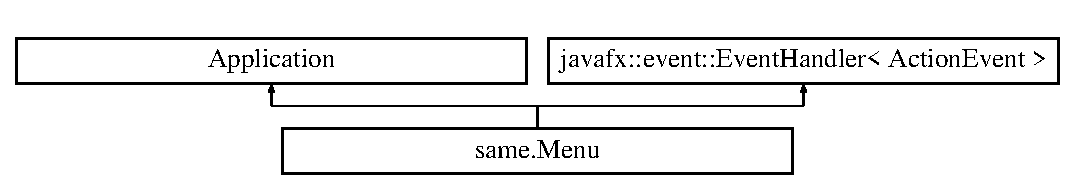
\includegraphics[height=2.000000cm]{classsame_1_1_menu}
\end{center}
\end{figure}
\subsection*{Public Member Functions}
\begin{DoxyCompactItemize}
\item 
void \hyperlink{classsame_1_1_menu_a6fa1dc5d1236ff823c8f137c30f086de}{start} (Stage primary\+Stage)  throws Exception 
\item 
void \hyperlink{classsame_1_1_menu_a5c930cf789ca6c4eee4dd807f451f75a}{handle} (Action\+Event evento)
\end{DoxyCompactItemize}
\subsection*{Static Public Member Functions}
\begin{DoxyCompactItemize}
\item 
\mbox{\Hypertarget{classsame_1_1_menu_af20b4178839b52c4ce23a26bd90cb76e}\label{classsame_1_1_menu_af20b4178839b52c4ce23a26bd90cb76e}} 
static void {\bfseries main} (String\mbox{[}$\,$\mbox{]} args)
\end{DoxyCompactItemize}
\subsection*{Public Attributes}
\begin{DoxyCompactItemize}
\item 
\mbox{\Hypertarget{classsame_1_1_menu_a8e989c6afc3b541638143c11f5b7bf7b}\label{classsame_1_1_menu_a8e989c6afc3b541638143c11f5b7bf7b}} 
int {\bfseries nivel} = 0
\end{DoxyCompactItemize}


\subsection{Member Function Documentation}
\mbox{\Hypertarget{classsame_1_1_menu_a5c930cf789ca6c4eee4dd807f451f75a}\label{classsame_1_1_menu_a5c930cf789ca6c4eee4dd807f451f75a}} 
\index{same\+::\+Menu@{same\+::\+Menu}!handle@{handle}}
\index{handle@{handle}!same\+::\+Menu@{same\+::\+Menu}}
\subsubsection{\texorpdfstring{handle()}{handle()}}
{\footnotesize\ttfamily void same.\+Menu.\+handle (\begin{DoxyParamCaption}\item[{Action\+Event}]{evento }\end{DoxyParamCaption})}

Accion de los botones 
\begin{DoxyParams}{Parameters}
{\em evento} & Variable que capta el evento de los botones\\
\hline
\end{DoxyParams}
\mbox{\Hypertarget{classsame_1_1_menu_a6fa1dc5d1236ff823c8f137c30f086de}\label{classsame_1_1_menu_a6fa1dc5d1236ff823c8f137c30f086de}} 
\index{same\+::\+Menu@{same\+::\+Menu}!start@{start}}
\index{start@{start}!same\+::\+Menu@{same\+::\+Menu}}
\subsubsection{\texorpdfstring{start()}{start()}}
{\footnotesize\ttfamily void same.\+Menu.\+start (\begin{DoxyParamCaption}\item[{Stage}]{primary\+Stage }\end{DoxyParamCaption}) throws Exception}

Metodo que inicia la interfaz gráfica 
\begin{DoxyParams}{Parameters}
{\em primary\+Stage} & El stage de la pantalla\\
\hline
\end{DoxyParams}


The documentation for this class was generated from the following file\+:\begin{DoxyCompactItemize}
\item 
src/same/Menu.\+java\end{DoxyCompactItemize}

%--- End generated contents ---

% Index
\backmatter
\newpage
\phantomsection
\clearemptydoublepage
\addcontentsline{toc}{chapter}{Index}
\printindex

\end{document}
